%! Author = breandan
%! Date = 2/3/22

% Preamble
\documentclass[11pt]{article}

% Packages
\usepackage{amsmath}
\usepackage{listings}
\usepackage{graphicx}


\lstset{
    basicstyle=\ttfamily,
    columns=fullflexible,
}

\title{COMP 764: High Level Synthesis}
\date{\today}
\author{Breandan Considine}
% Document
\begin{document}
    \maketitle

\section{VHDL generation}
\subsection{Simple test}

\begin{lstlisting}
RAM = malloc(4);
RAM[3] = RAM[0] * RAM[1] + RAM[2]
\end{lstlisting}

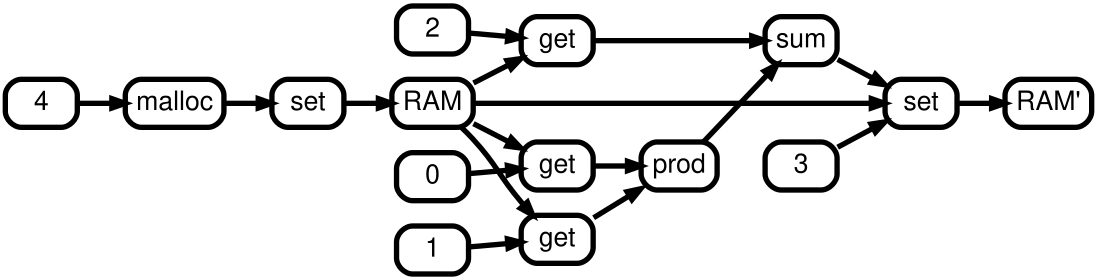
\includegraphics[scale=0.25]{rtd31}

\pagebreak\subsection{Vector multiplication}

\begin{lstlisting}
A = malloc(4);
B = malloc(4);
C = malloc(4);
C[0] = A[0] * B[0];
C[1] = A[1] * B[1];
C[2] = A[2] * B[2];
C[3] = A[3] * B[3];
\end{lstlisting}

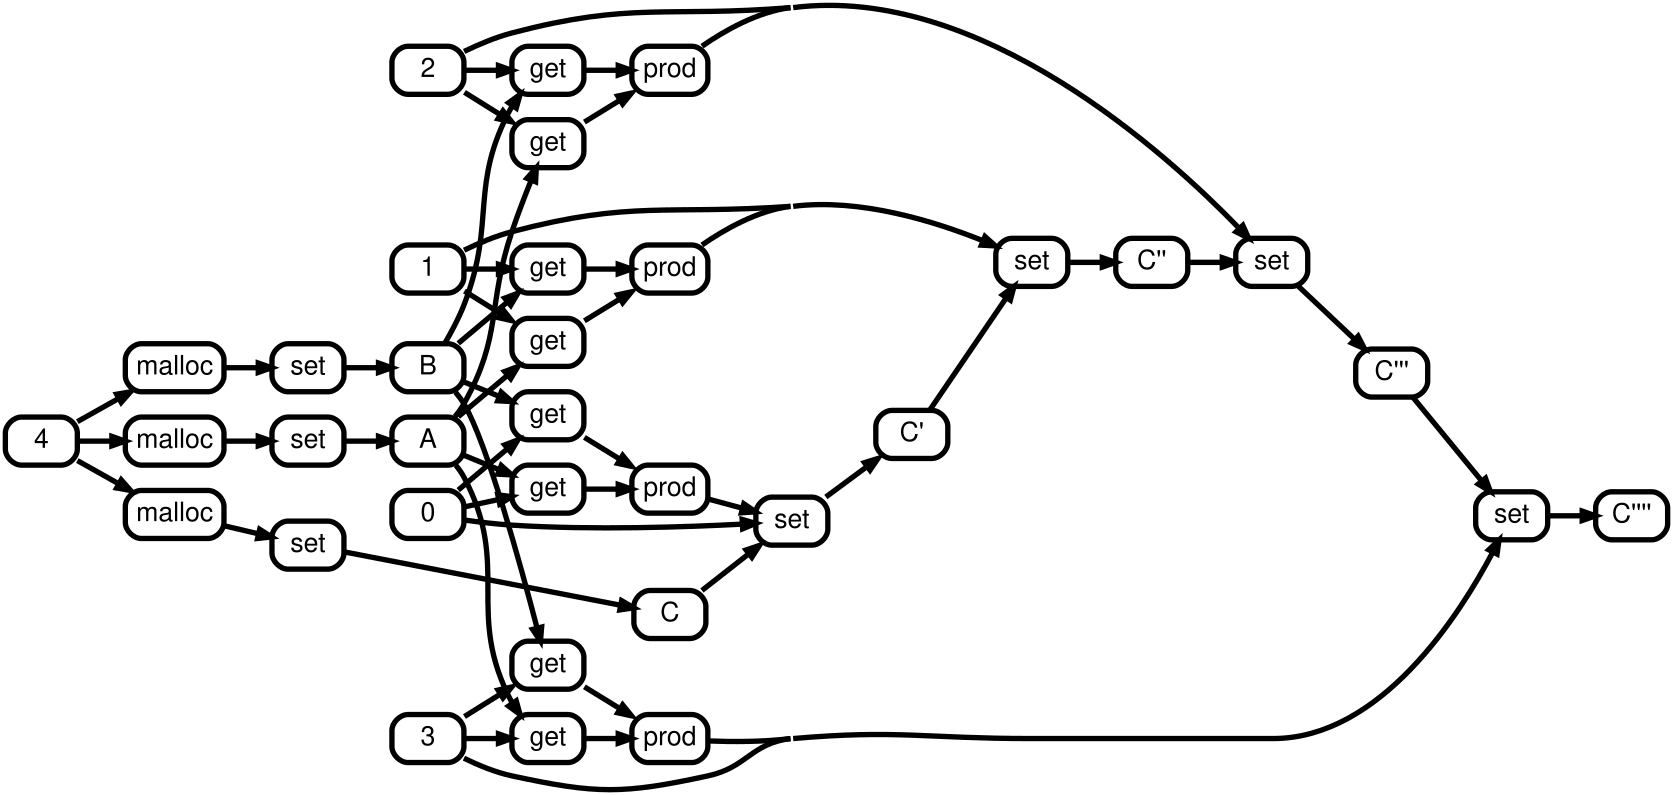
\includegraphics[scale=0.25]{rtd32}

\pagebreak\subsection{Dot product}

\begin{lstlisting}
A = malloc(4);
B = malloc(4);
C = malloc(1);
C[0] = A[0] * B[0] +
       A[1] * B[1] +
       A[2] * B[2] +
       A[3] * B[3];
\end{lstlisting}

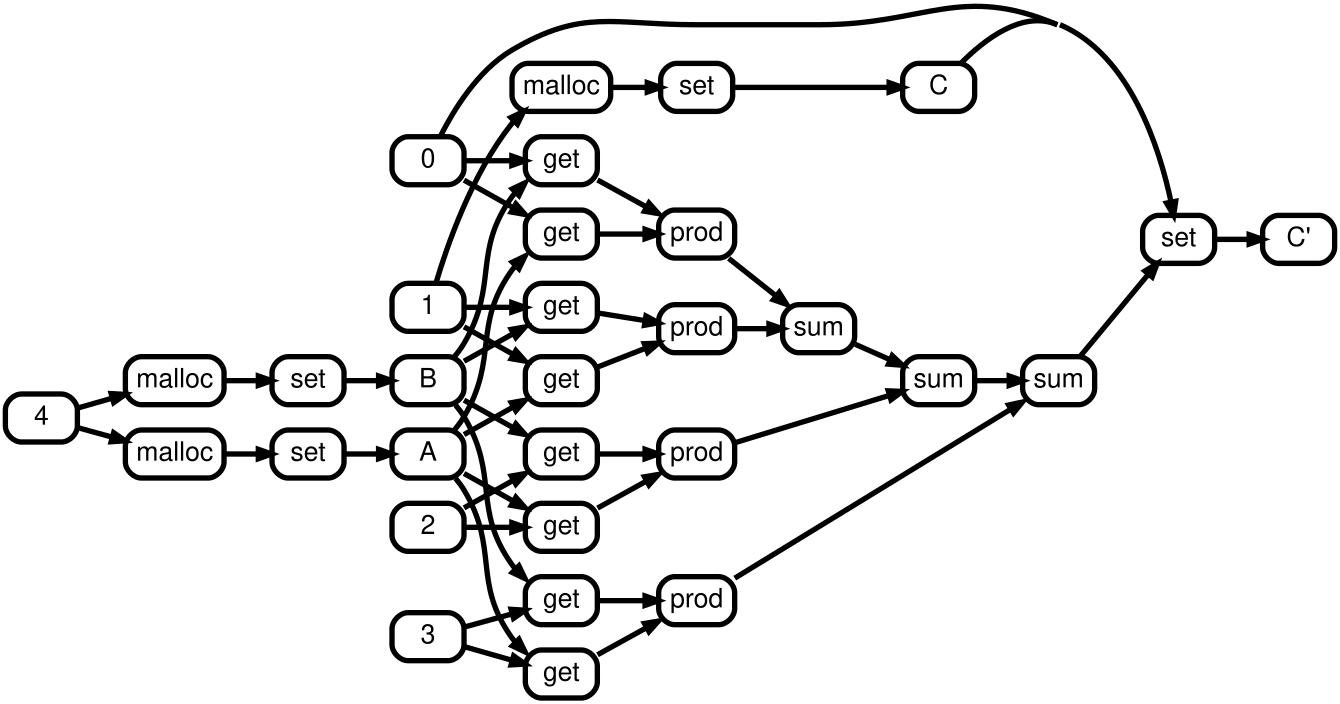
\includegraphics[scale=0.25]{rtd33}

\pagebreak\subsection{Convolution}

\begin{lstlisting}
A = malloc(6);
W = malloc(3);
C = malloc(4);
C[0] = A[0] * W[0] + A[1] * W[1] + A[2] * W[2];
C[1] = A[1] * W[0] + A[2] * W[1] + A[3] * W[2];
C[2] = A[2] * W[0] + A[3] * W[1] + A[4] * W[2];
C[3] = A[3] * W[0] + A[4] * W[1] + A[5] * W[2];
\end{lstlisting}

    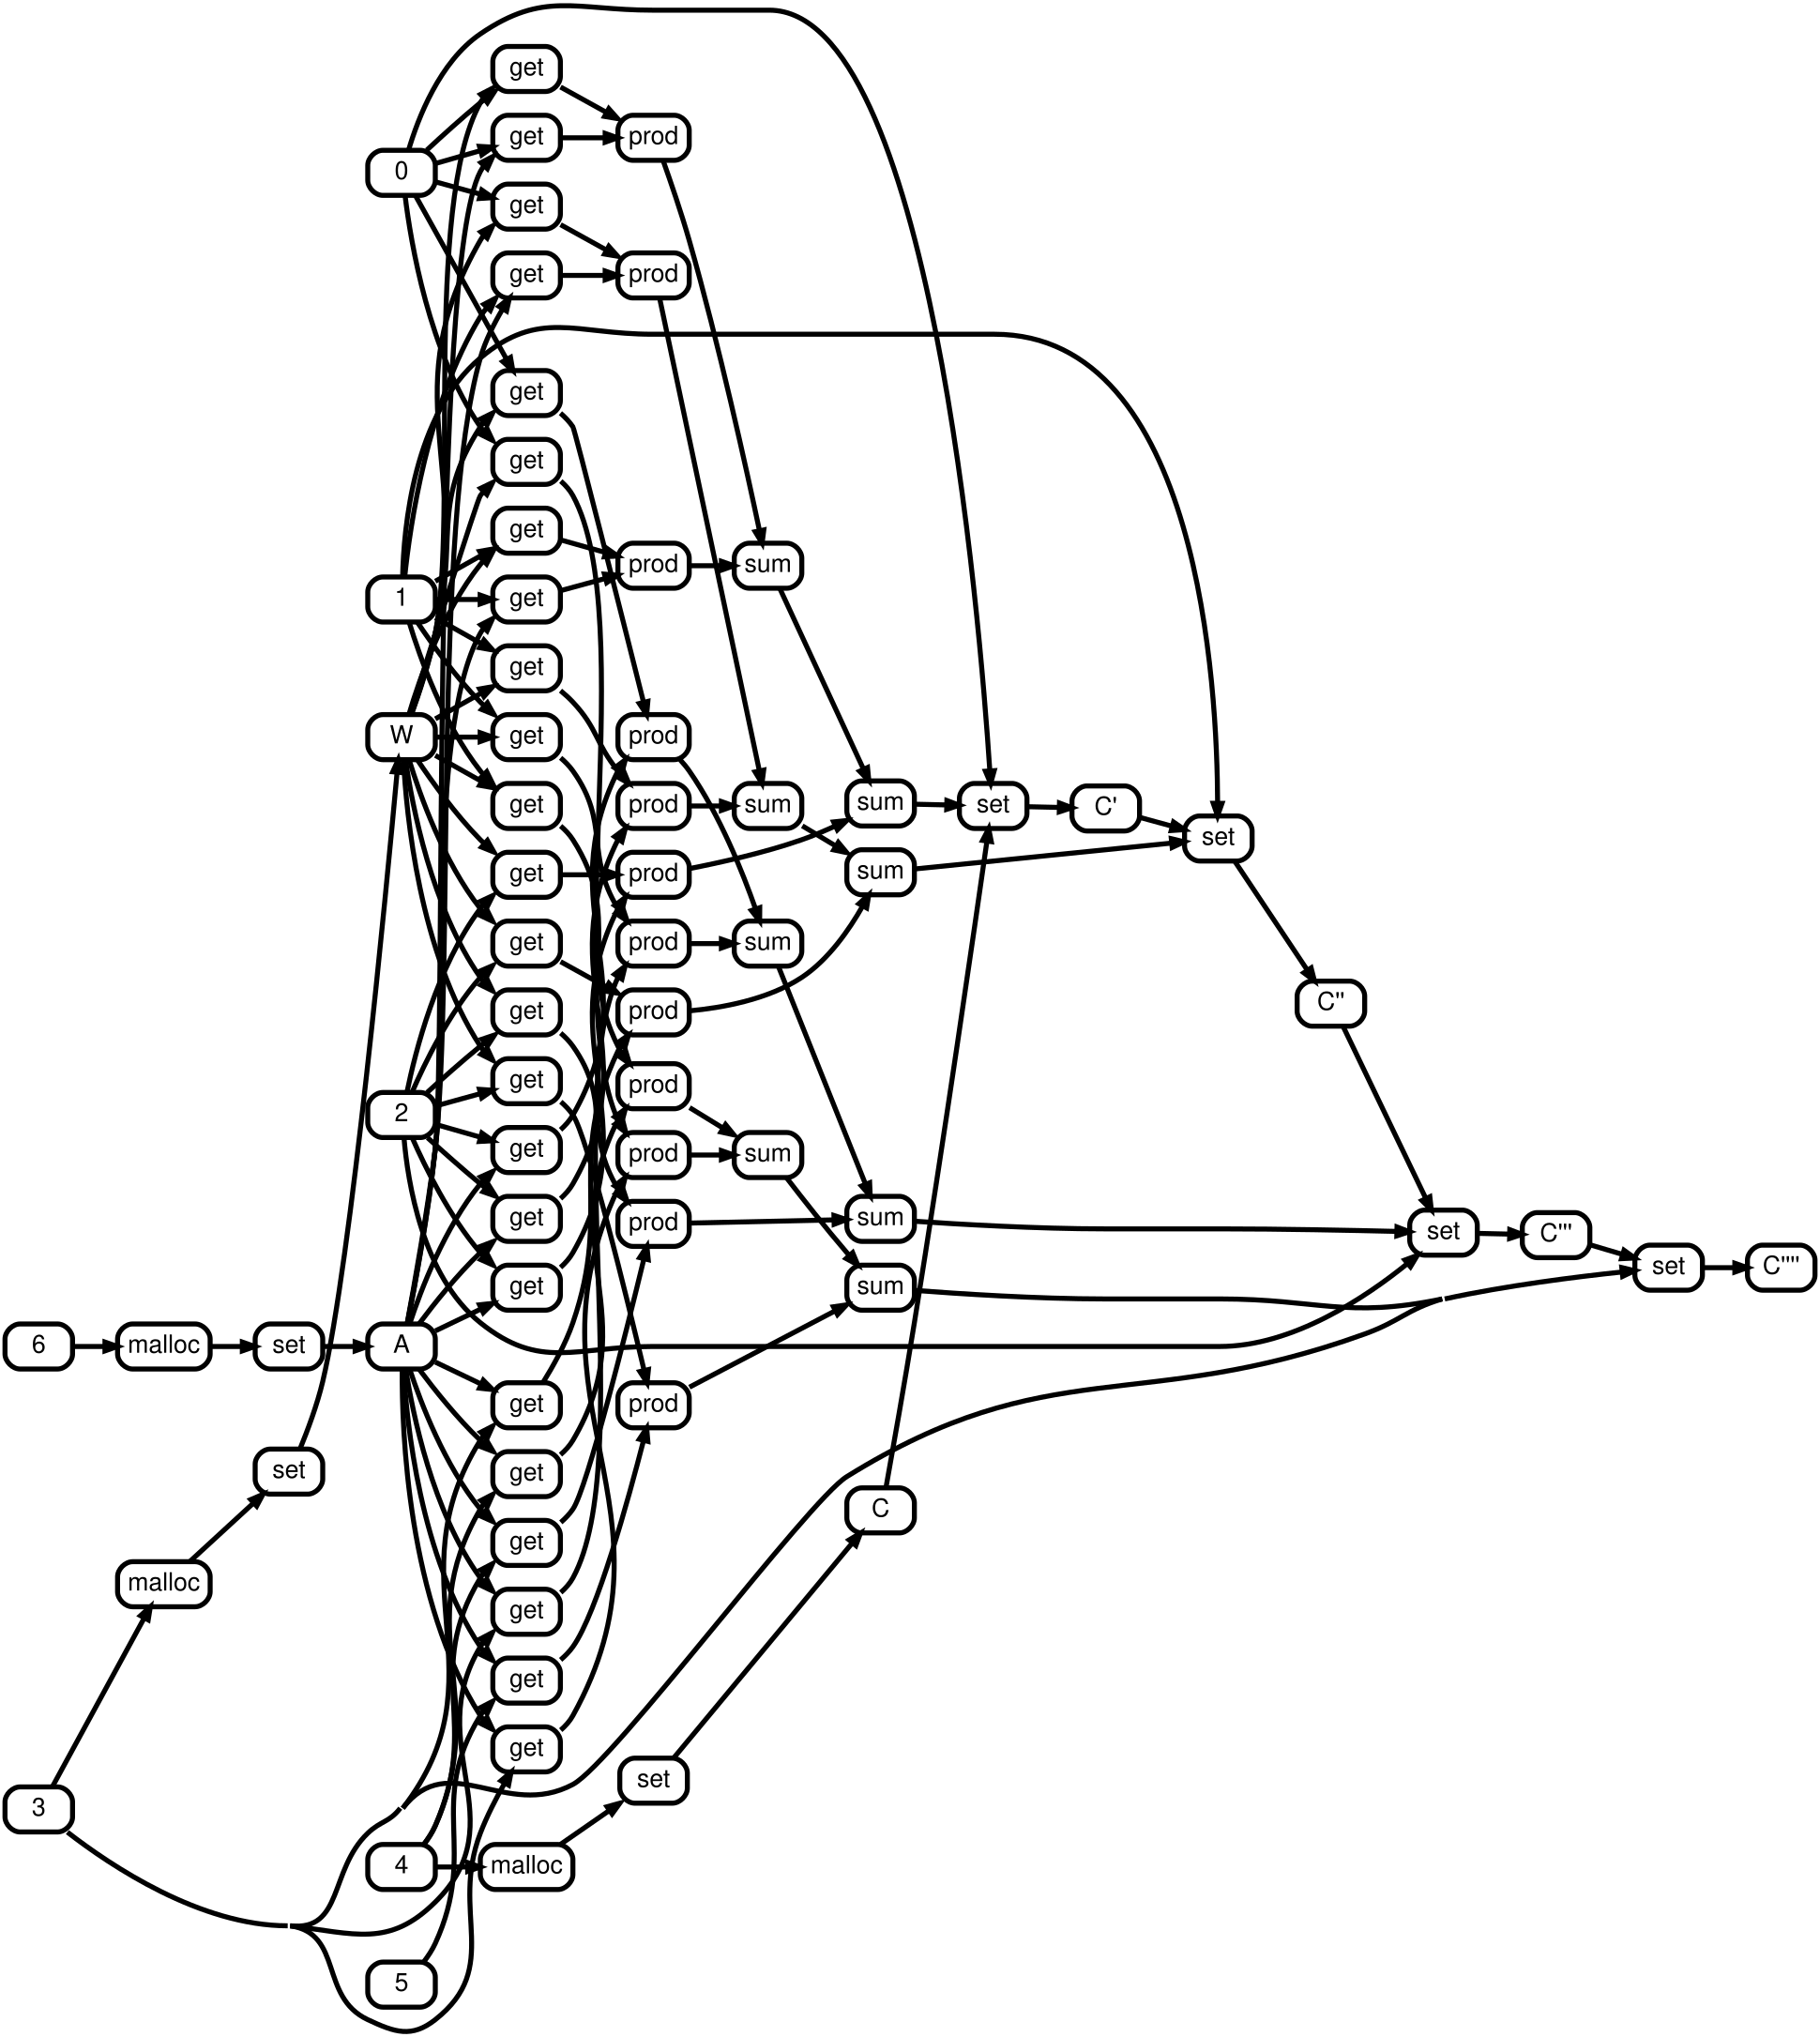
\includegraphics[scale=0.25]{rtd34}

\end{document}